\documentclass{article}

% ------ TEMPLATE ------ %

% ---------------------- %

% ------ PACKAGES ------ %

\usepackage{charter}
\usepackage{geometry}
\usepackage{amsmath}
\usepackage{amssymb}
\usepackage{float}
\usepackage{graphicx}
\usepackage{tabularx}
\usepackage{array}
\usepackage{subcaption}
\usepackage{enumitem}
\usepackage{titlesec}
\usepackage{hyperref}
\usepackage{xcolor}
\usepackage{pifont}
\usepackage{fancyvrb}
\usepackage{listings}
\usepackage{multirow}
\usepackage{ulem}
\usepackage{minted}

% ---------------------- %

% ------ GENERALS ------ %

\setlist[itemize]{label=\scriptsize\textbullet}
\setlist[itemize]{noitemsep, topsep=1pt}
\setlist[enumerate]{noitemsep, topsep=1pt}

\titleformat{\chapter}[hang]
{\normalfont\huge\bfseries}{\thechapter}{1em}{}
\titleformat{\subsubsection}{\large\bfseries}{\thesubsubsection}{1em}{}

% ---------------------- %

% ------- COLORS ------- %

\hypersetup{
    colorlinks=true,
    linkcolor=blue!50!black,
    urlcolor=blue,
    citecolor=blue,
    pdfborder={0 0 0}
}

% ---------------------- %

% ------ COMMANDS ------ %

\newcommand{\vmark}{\textcolor{teal}{\ding{51}}}
\newcommand{\xmark}{\textcolor{red!70!black}{\ding{55}}}
\newcommand{\newpar}[0]{\vspace{2mm}\noindent}
\newcommand{\htitle}[1]{\newpar\textbf{#1 -}}
\newcommand{\ititle}[1]{\newpar\hspace{1em}\textbf{#1}}
\newcommand{\hyperlabel}[1]{\hypertarget{#1}\phantomsection\label{#1}}
\newcommand{\hyperitem}[2]{\item \hyperlink{#1}{#2}\leaders\hbox to 0.8em{\hss.\hss}\hfill\hbox to 1.8em{\hss\pageref{#1}}}
\newcommand{\stdtilde}[0]{\raise.17ex\hbox{$\scriptstyle\sim$}}
\newcommand{\xor}[0]{\char`\^}
\newcommand{\saveformula}[2]{\newbox{#1}\savebox{#1}{#2}}
\newcommand{\useformula}[1]{\usebox{#1}}

% ---------------------- %

\begin{document}

% -------- HEAD -------- %

\pagenumbering{gobble}

\begin{center}

	\fontsize{20pt}{30pt}\selectfont
	Well MEing

	\vspace{2cm}

	\fontsize{25pt}{45pt}\selectfont
	\textbf{User Testing}

	\vfill

	\fontsize{12pt}{18pt}\selectfont
	Matteo Bettiati \\
	Lorenzo Bianchi \\
	Alessio Caggiano \\
	Francesco Ostidich \\
	Denis Sanduleanu \\

	\vspace{1cm}

	\today \\
	\vspace{12pt}
	Version: 1.0
	\normalsize

\end{center}

\newpage
\pagenumbering{arabic}
\tableofcontents
\newpage

% ---------------------- %

% -------- BODY -------- %

\section{Introduction}

This document outlines the user testing conducted on the Well MEing mobile application, designed to help users manage their well-being by tracking habits and metrics in a fully personalized manner.
Participants were asked to complete a series of tasks aimed at evaluating the application’s usability and functionality.
After each task, they filled out a form to provide feedback and rate the task’s difficulty on a scale from 1 to 5.
The collected feedback was then analyzed to identify areas for improvement and ensure the application effectively meets users’ needs.

\section{Task descriptions}

Before beginning the tasks, users received a brief introduction to the application, outlining its purpose and main features.
They then took each task one by one, and rated its difficulty from 1 to 5, where 1 corresponded to "Difficult to achieve" and 5 to "Easy and intuitive".

\subsection{Task 1: habit creation}

\begin{center}
	\textit{
		You want to track your "Run" habit: create the habit and select at least three metrics you like (e.g. distance, time, effort).
		Insert at least 2 different input types (slider, rating, time).
	}
\end{center}

The user is asked to create a new habit within the application.
This task evaluates the user's ability to navigate the interface and use the habit creation features.

\subsection{Task 2: habit logging with vocal assistant}

\begin{center}
	\textit{
		Simulate that you've come back from your "Run": insert all the data you chose to collect in task 1 using the vocal assistant.
	}
\end{center}

The user is asked to log an habit using the voice assistant.
This task assesses how easily the user can use voice commands to log habits without needing to enter data manually.

\subsection{Task 3: health from Apple}

\begin{center}
	\textit{
		Import, from Apple Health, some habits you are interested to track (at least 2).
	}
\end{center}

The user is asked to connect the app with Apple Health and retrieve health data.
This task tests the user’s ability to integrate external health data into the app.

\subsection{Task 4: report creation}

\begin{center}
	\textit{
		Request a report about you "Run" habit.
	}
\end{center}

The user is asked to generate a report based on their tracked habits and health metrics.
This task evaluates how well the user can review and analyze their progress over time.

\subsection{Task 5: data visualization}

\begin{center}
	\textit{
		Take a look at your submissions by reviewing the charts and the calendar, at today's date.
	}
\end{center}

The user is asked to view visual representations of their habit and health data.
This task assesses the user's ability to interpret the charts and understand their progress.

\subsection{Task 6: removing data}

\begin{center}
	\textit{
		Choose some data, it being a whole habit, a submission in the calendar or a report and delete it.
	}
\end{center}

The user is asked to delete an habit along with all its associated data.
This task checks how effectively the user can manage and remove personal data from the app.

\section{Results analysis}

The results of the user testing are summarized in the following sections, which showcase the perceived average difficulty rating for each task.

\subsection{Task 1: habit creation}

\begin{center}
	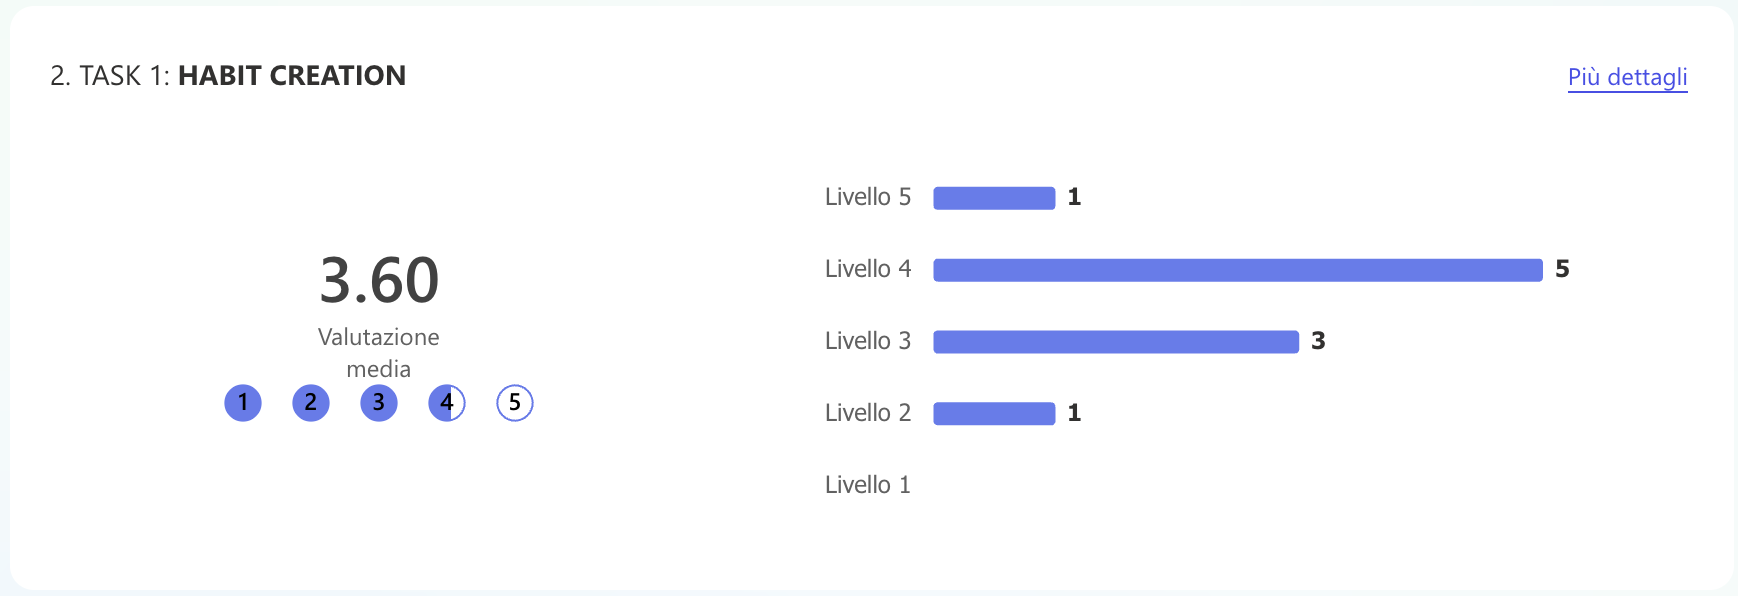
\includegraphics[width=\linewidth]{images/habit-creation-result.png}
\end{center}

\subsection{Task 2: habit logging with vocal assistant}

\begin{center}
	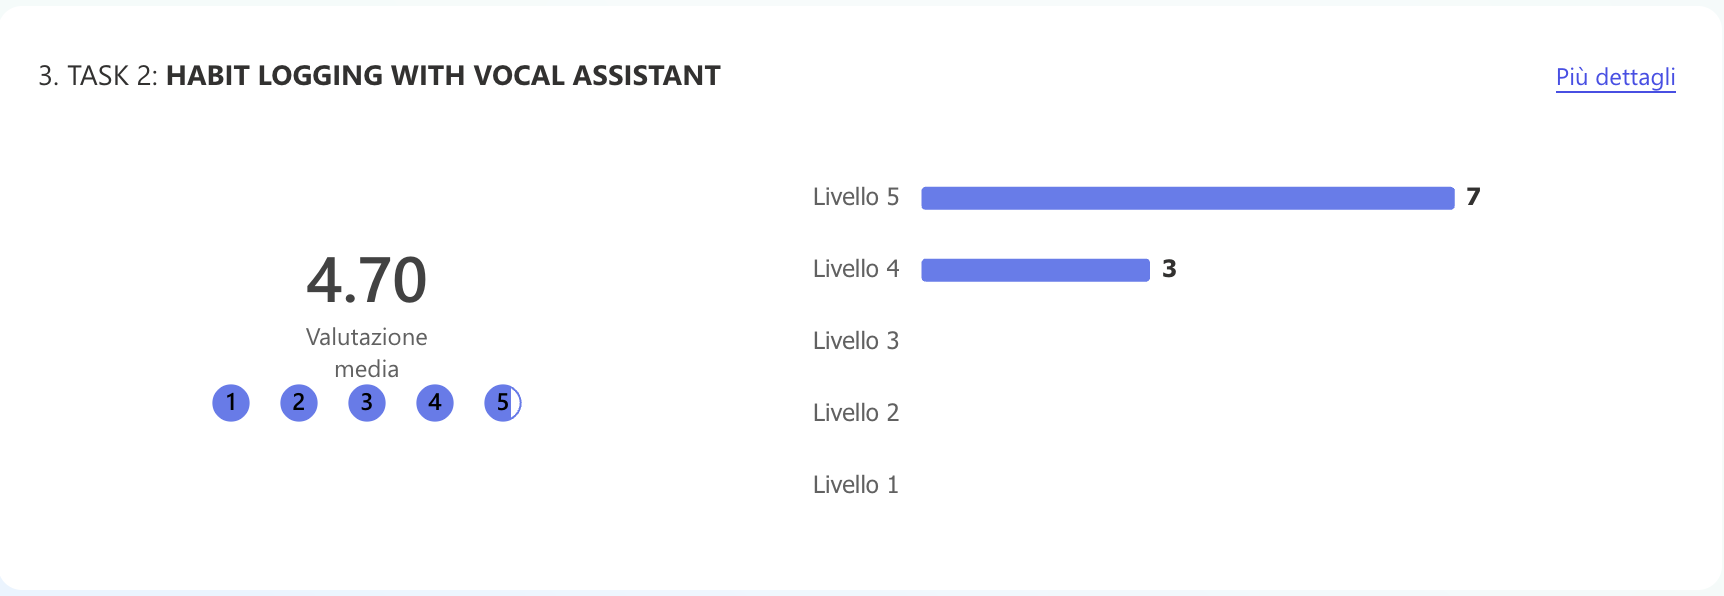
\includegraphics[width=\linewidth]{images/habit-logging-with-vocal-assistant-result.png}
\end{center}

\subsection{Task 3: health from Apple}

\begin{center}
	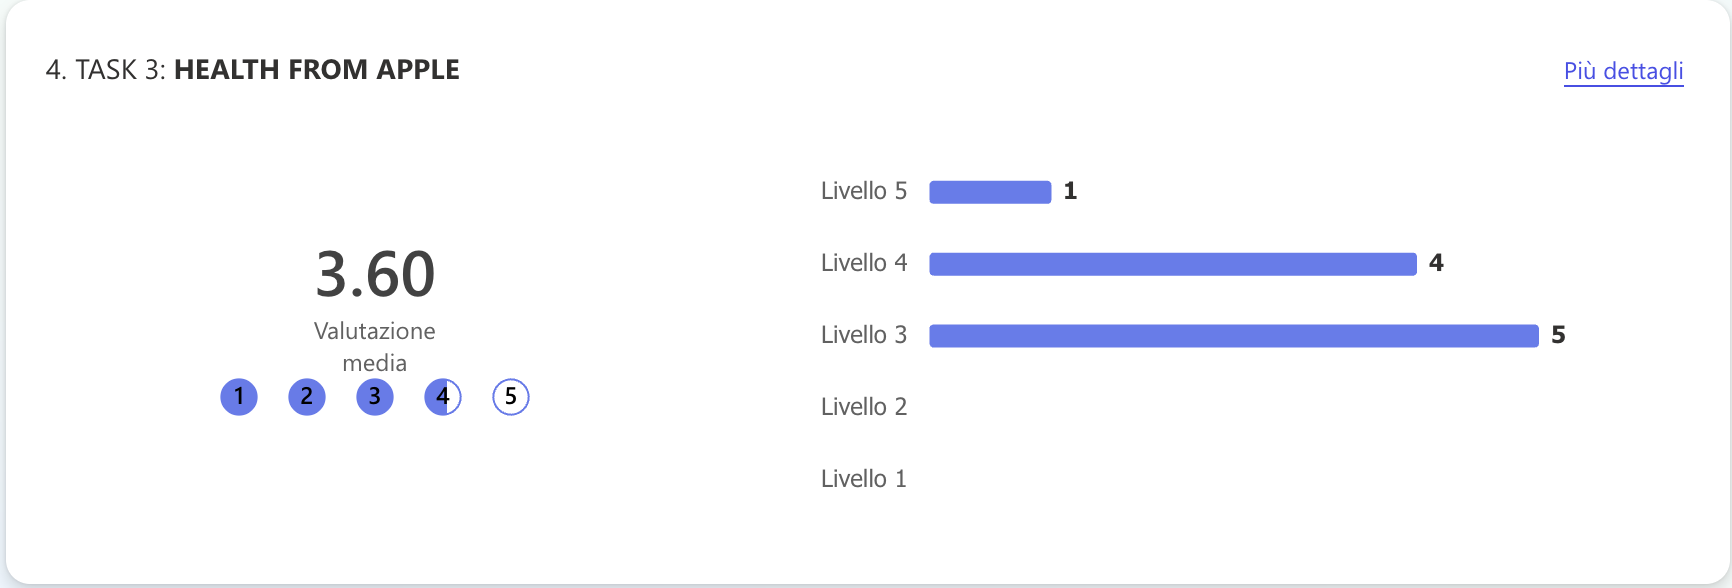
\includegraphics[width=\linewidth]{images/health-from-apple-result.png}
\end{center}

\subsection{Task 4: report creation}

\begin{center}
	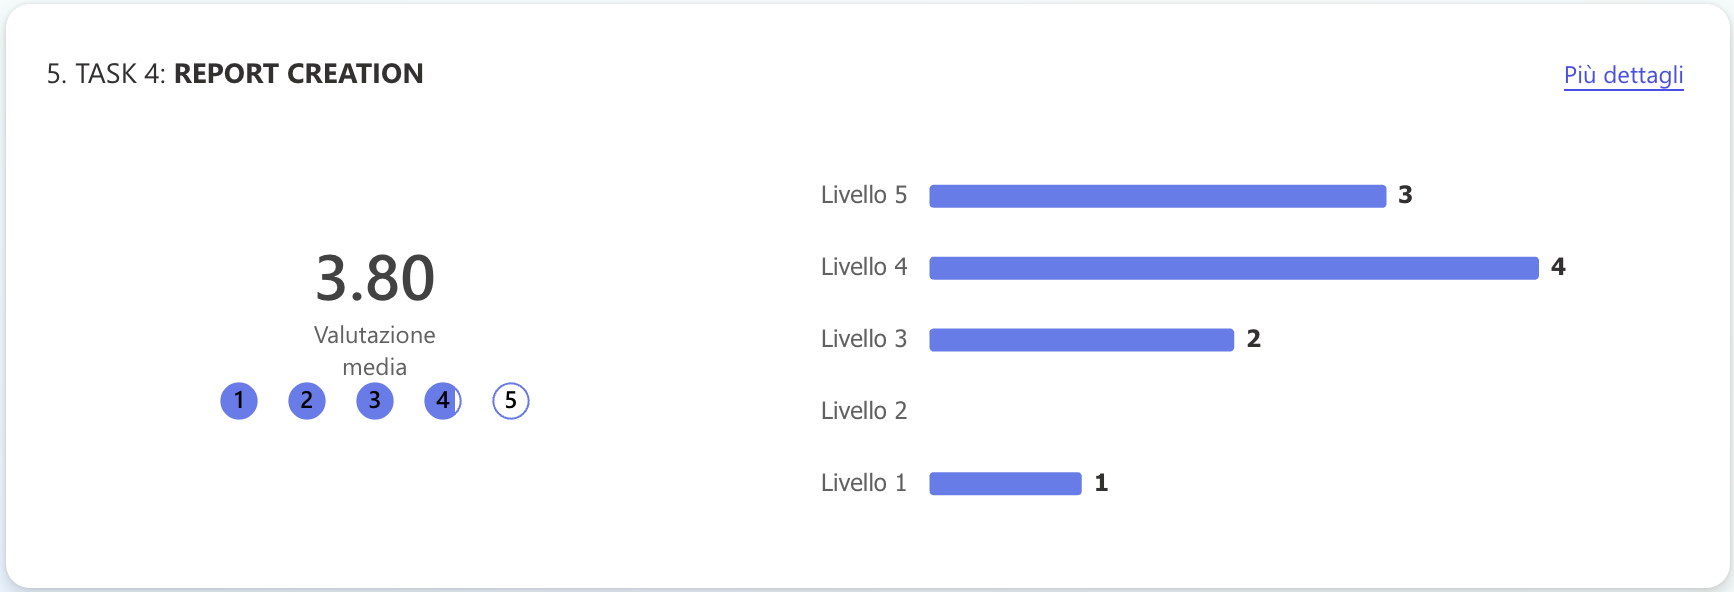
\includegraphics[width=\linewidth]{images/report-creation-result.png}
\end{center}

\subsection{Task 5: data visualization}

\begin{center}
	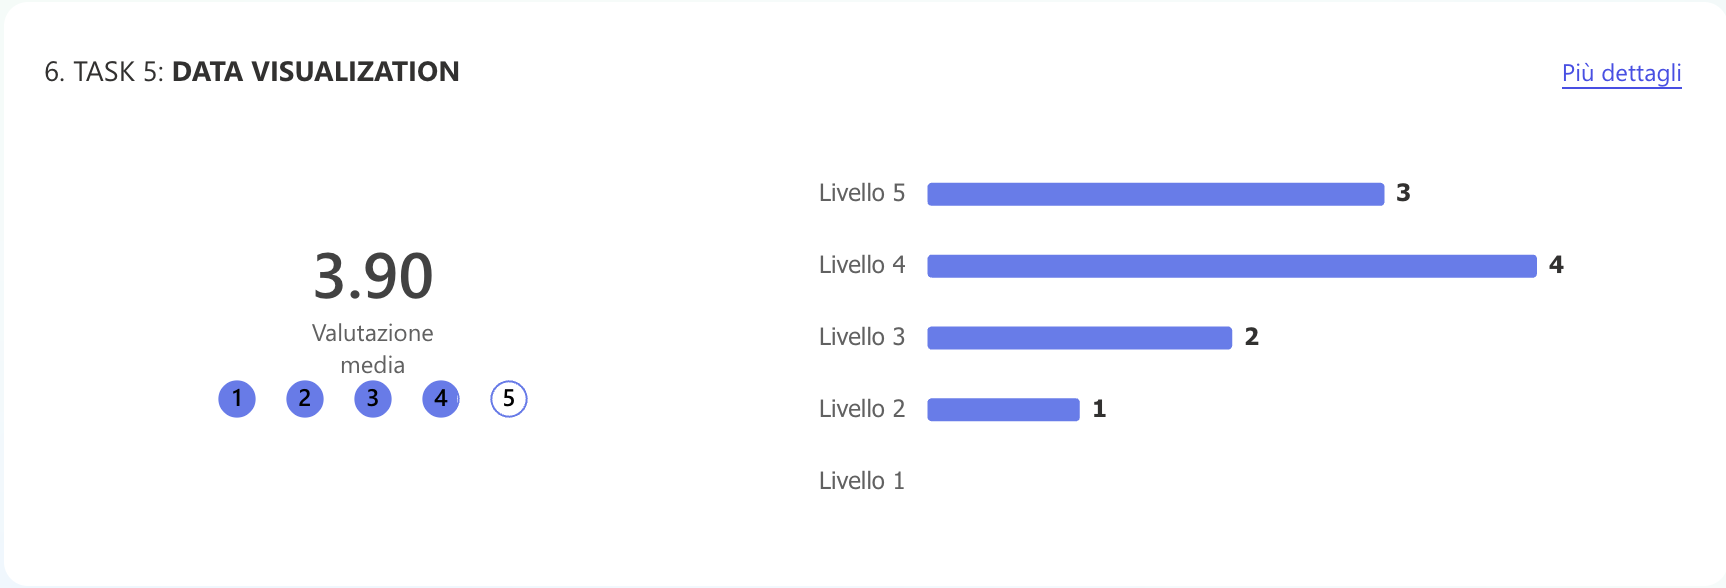
\includegraphics[width=\linewidth]{images/data-visualization-result.png}
\end{center}

\subsection{Task 6: removing data}

\begin{center}
	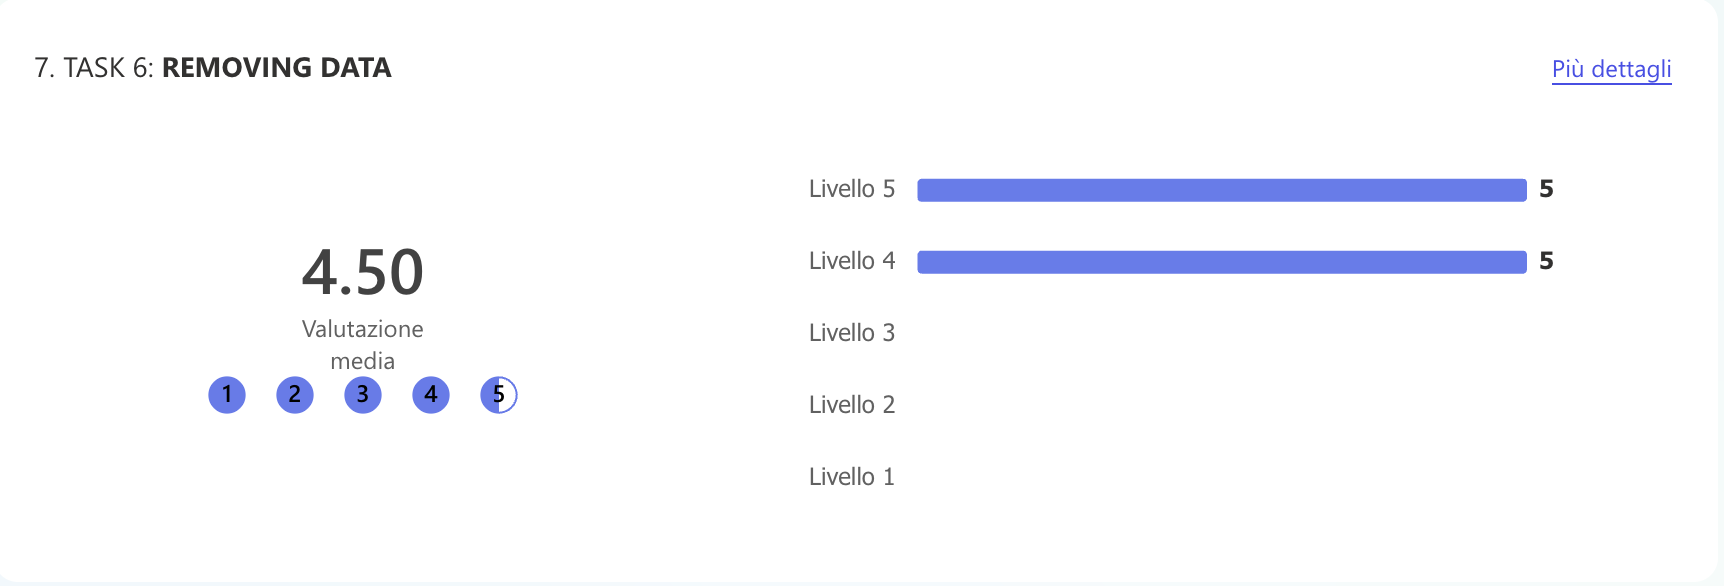
\includegraphics[width=\linewidth]{images/removing-data-result.png}
\end{center}

\section{General impressions}

Overall, users find the application well-made and thoughtfully designed.
The features are well-distributed, and the color scheme aligns well with the app's core concept, providing everything needed for its intended purpose.

Some of the aspects that received a positive feedback are listed here after.

\begin{itemize}
	\item \textbf{Effective statistics and reports}: the statistics and report sections are considered perfect and very well done, indicating strong performance in data analysis and presentation.
	\item \textbf{Convenient deletion and data import}: the delete function is quick and convenient, and the ability to import data from Apple Health is highly appreciated and deemed very useful.
	\item \textbf{Promising voice feature}: the voice functionality was liked, showing potential for efficient interaction, particularly for quick tracking.
\end{itemize}

\section{Areas for improvement}

While the app has many strengths, some areas could be refined to enhance the user experience.

\subsection{Onboarding and clarity}

\begin{itemize}
	\item \textbf{Main page clarity}: the main page functionalities aren't immediately clear, making it hard for new users to understand what each option does; renaming options, such as "Import Health" to "Import Apple Health," could help.
	\item \textbf{Data import process}: the process for uploading data in the "Import Health" page needs to be clearer; additionally, users expect the app to automatically import historical data when an activity is first imported, rather than allowing the selection of the current data only.
\end{itemize}

\subsection{Habit creation and management}

\begin{itemize}
	\item \textbf{Habit modification}: users desire the ability to modify habits after creation (e.g., correcting spelling errors) to ensure accuracy over time.
	\item \textbf{Confusing interactive preview}: the interactive preview of metrics during habit creation is confusing; users find difficult to understand the purpose of the input requested.
\end{itemize}

\subsection{Visualization and navigation}

\begin{itemize}
	\item \textbf{Calendar integration}: users would like to manage habit entries directly from the calendar.
	\item \textbf{Calendar visual cues}: adding colored dots to same habits in the calendar, to quickly visualize habit entries on specific days (and distinguishing between multiple habits on the same day), would greatly improve glanceability.
\end{itemize}

Feedbacks suggested a strong foundation for the app, but with clear opportunities to enhance user intuition, flexibility, and visual clarity, especially in habit management and data presentation.

\section{Feedback raw data}

Here is shown the plain textual feedbacks received in the form.

\begin{itemize}
	\item I think the application is very well-made: the features are well-distributed, colors are "in line" with the main concept, and it has everything needed to fulfill its purpose. However, I encountered some problems. During the creation phase, some metrics are counterintuitive, and certain data, like goals, can only be set at the beginning and therefore aren't modifiable during normal use. In general, I think being able to modify an habit could be convenient (for example, if you realize you made a spelling error only after adding progress). The statistics phase, however, is perfect. The data import phase is very useful, but I think it could be improved regarding the actual import of activity. That is, when I first import an activity, I expect it to automatically import all data up to that moment. The report phase, however, is very well done.
	\item I found the delete function quick and convenient, as well as the ability to import data from Apple Health. I would have liked the ability to manage habit entries directly from the calendar.
	\item I would have preferred to have the week selection below the data visualization charts because the arrows get confused with the arrows for changing the data being displayed. Additionally, it would be better to add dots on the calendar to quickly see if habits were entered on that specific days (using different colored dots if two different habits were entered on the same day).
	\item The main page isn't very clear; at first glance, it's hard to understand what each option does. For example, "Import Health" could be "Import Apple Health." On the Import Health page, it's not clear how to upload your data to the app. When creating habits, there's an interactive preview of metrics that I find very confusing for a user who sees an input request and doesn't quite understand what to do with it. I don't understand why you can't enter a number without a slider (I know there's generic text input, but it's not a very intentional option). In the progress page, I find it difficult to visualize which habit, which session, and which metrics are being displayed. I can't think of a good alternative solution right off the bat, but in my opinion, it needs revisiting since I think it's the most important part to track what you've done well and quickly. I really like the voice feature, even though it's not clear what it's capable of doing and what it's not. In general: the GUI itself isn't bad, but I don't really like the design. The functionalities are nice, but personally, I'd use an app like this primarily for quick tracking and visualization. For voice tracking, we're there, but for visualization, other solutions could be explored.
	\item Make more clear after vocal interactions that you have to submit. A tutorial is needed.
	\item Renaming requires double clicking. Form in calendar are not intended to be shown. Calendar could highlights dates with submissions. Deletion is not obvious.
\end{itemize}

\end{document}
